\vspace{0.015\textheight}
In order to understand how particles are produced and how they interact, one needs to study the actual physics process occurring at the interaction point. To do this, the particles produced in a \ppbar interaction are used to infer the original physics process. The produced particles, as they traverse the detector, interact with it and generate electronic signals. Those electronic signals are used to recreate the particles' properties, such as their energies and momenta, as well as the location of the interaction point. From this information, the actual interaction can be completely reconstructed. The process of converting electronic signals into particles that can be used in physics analyses is called \newterm{event reconstruction}. In this chapter, the reconstruction and identification of photons, electrons, and jets are described in detail. This chapter also describes the energy corrections to the measured jets. Finally, definitions of several kinematic quantities measured in the analysis are given.

\section{Photon Identification}\label{sec:photon_identification}

In order to identify a photon, information from various subdetector components is combined using the following general procedure.  First, individual detector segments (towers, wires, or scintillator tiles) that have a signal above a predetermined minimum threshold are identified.  Then, the qualifying segments are grouped to form \newterm{clusters}. The formation of the clusters is tuned and optimized in each type of subdetector component based on its design. In most situations, iterative algorithms are used to identify and form these clusters. The final measurement of the photon is done based on this clustered energy.

\subsection{Calorimeter Energy Clustering}
Calorimeter towers containing energy deposited by photons produced in the hard scattering process are grouped to form energy clusters via a clustering algorithm. First, the whole detector is searched for towers with a transverse energy above a minimum threshold ($\sim$100~MeV), and these towers are considered in the clustering process. The towers are sorted by decreasing \et and seed towers with $E_{T}>3$~GeV are selected. Finally, towers within a rectangular grid ($3\times 3$) around the seed towers are considered for inclusion in the EM clusters. The grid size is reduced to $2\times 2$ in the plug calorimeter photon reconstruction to reduce effect of jets. Energy in a cone of radius $\Delta R=\sqrt{\Delta\eta^{2}+\Delta\phi^{2}}=0.4$ (see Fig.~\ref{fig:PhotonIsoCone}), centered on the seed tower, generally should include almost all of the energy of a single photon or electron. Initial EM clustering is always done assuming the primary interaction is located at $x=y=z=0$ \cite{cdfnote:5456}. (This is also true for clustering jets.)

\begin{figure}[htb!]
 \centering
 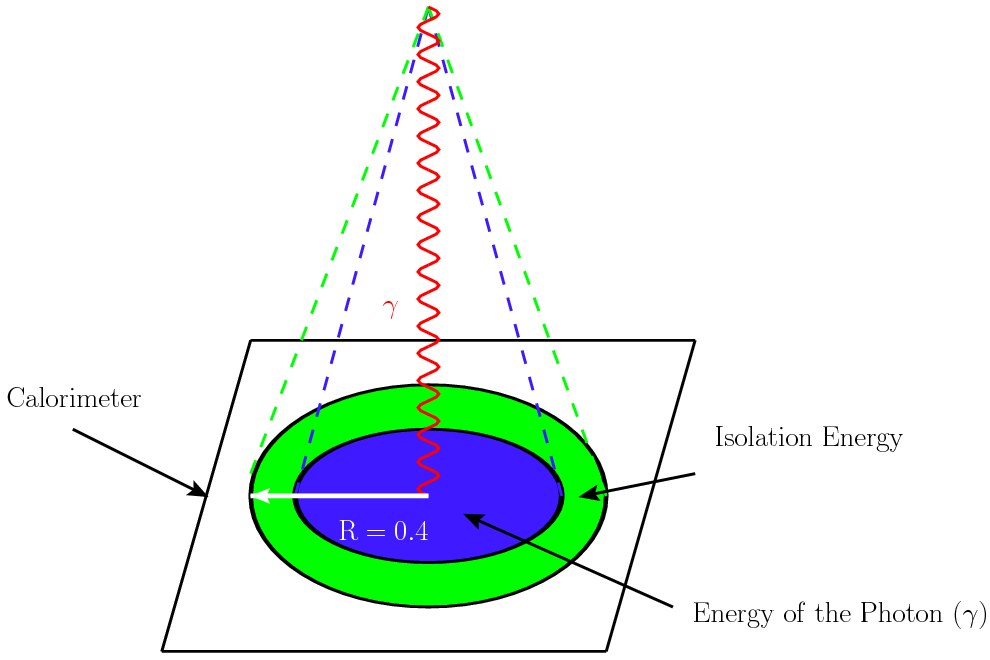
\includegraphics[scale=0.35,keepaspectratio=true]{./PhotonIsolationDemo.png}
 \caption{A geometric cone is used to reconstruct a photon in the detector. Reconstruction requires the photon to be isolated by limiting the extra energy surrounding it.}
 \label{fig:PhotonIsoCone}
\end{figure}

The total energy ($E$) of the cluster includes the sum of the energies of the EM ($E_{EM}$) and HAD ($E_{HAD}$) calorimeters. The coordinates of the EM cluster are initially derived by an energy-weighted method as described below.

First, $\eta_{EM}$ and $\phi_{EM}$ are calculated using the EM towers in the cluster and $\eta_{HAD}$ and $\phi_{HAD}$ using the HAD towers in the cluster.
\begin{eqnarray}
 \eta_{EM} &=& \frac{\sum_{i}E^{i}_{EM}\cdot\eta^{i}}{\sum_{i}E^{i}_{EM}}\\
 \phi_{EM} &=& \frac{\sum_{i}E^{i}_{EM}\cdot\phi^{i}}{\sum_{i}E^{i}_{EM}}\\
 \eta_{HAD} &=& \frac{\sum_{i}E^{i}_{HAD}\cdot\eta^{i}}{\sum_{i}E^{i}_{HAD}}\\
 \phi_{HAD} &=& \frac{\sum_{i}E^{i}_{HAD}\cdot\phi^{i}}{\sum_{i}E^{i}_{HAD}}
\end{eqnarray}
Then the actual coordinates are calculated using
\begin{eqnarray}
 \eta &=& \frac{E_{EM}\cdot\eta_{EM}+E_{HAD}\cdot\eta_{HAD}}{E}\\
 \phi &=& \frac{E_{EM}\cdot\phi_{EM}+E_{HAD}\cdot\phi_{HAD}}{E}
\end{eqnarray}
Finally, the energy of the (photon) cluster is corrected by measuring its position in the CES with respect to the primary vertex. Then, using the polar angle ($\theta$), the transverse energy of the photon cluster can be calculated using
\begin{equation}
 E_{T} = E\cdot\mathrm{sin}(\theta)
\end{equation}

\subsection{CES Energy Clustering}
There are two types of CES energy clustering algorithms; one is \newterm{track-based} and the other is \newterm{strip-based}.

The \newterm{strip-based} or \newterm{unbiased} CES clustering sorts the strips/wires by decreasing energy and seeds the cluster with the highest energy strip. Then, a strip/wire collection is formed by gathering $N$ strips around the seed, where $N$ is a tunable parameter. All the strips belonging to clusters are tagged and removed from the remaining collection of strips. Hence, a strip cannot belong to two clusters, unlike in the track-based clustering. This clustering method is specifically designed for photon identification.

The \newterm{track-based} algorithm, which is designed mostly for charged electromagnetic particles (i.e.~for electrons), finds the seed of the cluster by extrapolating a track to the CES radius. Then it records the $x$ and $z$ coordinates of the track in the CES local coordinate system. Finally, it forms a strip collection by finding the strip that is hit and adding $N$ number of strips around the seed strip where $N$ is a tunable parameter. The result is that all the tracks in an event passing some minimum quality selection requirements are associated with a CES cluster.

\subsection{Photon Selection Requirements}
A combination of kinematic and fiducial selection requirements are applied sequentially to the EM clusters to identify photon candidates. Offline calibration and calorimeter energy scale corrections are applied to the calorimeter energy cluster. The standard photon selection requirements include a minimum corrected transverse energy (\etcorr) greater than \etg{7}. The CES fiducial selection requirements make sure the cluster (shower) is contained within the instrumented regions of the detector. The CES shower position is determined by the \et-weighted centroid of the highest energy clusters of those strips and wires in the CES that correspond to the seed tower. The direction of the photon can be inferred by connecting the primary event vertex and the CES shower position. Being an electromagnetic object, photons are expected to lose all of their energy inside the EM calorimeter. The selection requirement, $E_{HAD}/E_{EM}$, the ratio of the total energy in the hadron calorimeter to the total energy in the EM calorimeter, is derived from this basic idea. This limits the number of jets identified as photons (or electrons). The presence of a track or tracks is used to distinguish photons from leptons and jets. At most one reconstructed track is allowed, and the \pt of that track should be small. This allows an increase in efficiency that otherwise would be lost due to a random low-\pt track from the underlying event. The isolation energy requirement further suppresses the lepton and jet backgrounds and is the most effective requirement for removing jets.
The variables used for photon identification are presented below together with the standard tight and loose photon selection requirements. Table~\ref{tab:tightAndLoosePhotonCuts} has a summary of the selection requirements. The photon candidate energy is corrected for the calorimeter energy response, the underlying event, and multiple interactions.

\begin{table}[p]
\caption{Standard Tight and Loose Photon selection requirements.}
\label{tab:tightAndLoosePhotonCuts}
\centering
\begin{tabular} {ccc}
\hline
\BUbf{Selection Variable} 	& \BUbf{Standard Requirement} & \BUbf{Loose Requirement}\\
\hline
detector ($\eta^{detector}$) 	& \etalessthan{1.1} & \etalessthan{1.1}\\
$\etcorr$ 	& \etg{30}	& \etg{30} \\[2ex]
CES X and Z & $ |X_{CES}| \leq 21 $ cm 	& $ |X_{CES}| \leq 21 $ cm\\
 fiducial & 9 cm $ \leq |Z_{CES}| \leq 230 $ cm 	& 9 $\leq|Z_{CES}|\leq230$ cm\\[2ex]
\multirow{2}{*}{$E_{HAD}/E_{EM}$} & $\leq 0.125$ & \multirow{2}{*}{$<$ 0.125}\\
& $|| \leq 0.055 + 0.00045 \times \ecorr$&\\[2ex]
\multirow{4}{*}{\isoetcorr in cone 0.4}
& $\leq 0.1 \times \etcorr$ & $\leq 0.15 \times \etcorr$ \\
 & if $\etcorr<20$~\etUnits & if $\etcorr<20$~\etUnits\\
 & $\leq 2.0 + 0.02 \times (\etcorr -20)$ & $\leq 3.0 + 0.02 \times (\etcorr -20)$ \\
 & if $\etcorr>20$\etUnits & if $\etcorr>20$\etUnits\\[2ex]
average CES $ \chi^2$	& \multirow{2}{*}{$\leq 20 $} & No selection\\
(Strips+Wires)/2 & & requirement \\[2ex]
N tracks in cluster& \multirow{2}{*}{$\leq1$} & \multirow{2}{*}{$\leq1$} \\
 (N3D)\\[2ex]
Track $\pt$ 	& $< 1+0.005 \times \etcorr$ 	& $<0.25 \times \etcorr$\\
Track Iso($0.4$) & $< 2.0 + 0.005 \times \etcorr $ & $<5.0$\\[2ex]
\multirow{4}{*}{}
$E_{T}$ of the 2\superscript{nd} CES cluster &if $\etcorr<18$~\etUnits & \multirow{4}{*}{No Requirement}\\
(both wire and & $\leq 0.14\times\etcorr$ & \\
strip) & if $\etcorr\geq18$~\etUnits & \\
 & $ \leq2.4+0.01\times\etcorr$ & \\
\hline
\end{tabular}
\end{table}
%%%%%%%%%%%%%%%% END TIGHT PHOTN ID CUTS %%%%%%%%%%%%
%%%%%%%%%%%%%% LOOSE PHOTON CUT %%%%%%%%%%%%%
%\begin{table}[hbm]
%\begin{center}
%\begin{tabular} {|c|c|}
%\hline
%\BUbf{Selection Variable} 		& \BUbf{Requirement} 	\\
%\hline
%detector 		 	& central 	\\
%\hline
%$\etcorr$ 	& $ >30 $ GeV \\
%\hline
%CES X and Z fiducial 		& $ |X_{CES}| \leq 21 $ cm \\
%				& $ 9 $ cm $ \leq |Z_{CES}| \leq 230 $ cm \\
%\hline
%Had/EM 		&	$ \leq 0.125$ \\
%\hline
%\isoetcorr in cone 0.4	& $\leq$ 0.15 $\times \etcorr$ if $\etcorr<$20 GeV\\
%					& $\leq$ 3.0 if \etcorr$>$20 GeV \\
%\hline
%Track $\pt$ 	& $< 0.25 \times \etcorr$ \\
%\hline
%Track Iso($0.4$) &	$< 5.0 $ \\
%\hline
%\end{tabular}
%\end{center}
%\caption{Loose Photon selection requirements.}
%\label{tab:loosephotoncuts}
%\end{table}
%%%%%%%%%%%%%% END LOOSE PHOTON CUTS %%%%%%%%
\vspace{-0.01\textheight}
\begin{singlespace}
\begin{itemize}
\item {\cutVar{Detector} Pseudorapidity ($\eta^{detector}$) --- This is the detector region where the object is found. The CDF detector is divided into three regions: central, plug, and forward. The central part lies within \etalessthan{1.1} and the plug region extends from \etaabsregion{1.1}{3.5}. The forward region extends from \etaabsregion{3.5}{5.9} (see Fig.~\ref{fig:TrackingCoverage}). The central part of the detector is better instrumented and well understood compared to the other two regions.
}

\item{$E_{T}= E \times \mathrm{sin}(\theta)$ where $E$ is the electromagnetic energy of the cluster and $\theta$ is the polar angle. This is the transverse component of energy deposited by a photon in the calorimeter. Standard selection rules require $E_{T}>7$~GeV to qualify as a photon candidate. (As photons are massless, $\et=\pt$.)
}

\item{CES Fiducial ($X_{CES}$, $Z_{CES}$) --- The CES requirements are defined by the active region of the detector. Requiring an energy deposition in an area covered by both strips and wires ensures that the energy cluster is well contained within the instrumented regions of the detector. The fiducial region is defined by the CES local coordinates $|x|<21$ cm and 9~cm~$<|z|<$~230~cm. The CES wire (strip) clusters are formed from an 11-wire (strip) window around the highest-\et seed wire (strip). The highest-\et wire (strip) must be within 25~cm in $z$ of the EM centroid.
}

\item{Average CES $\chi^2$ --- The $\chi^2$ value is a measure of the shape of the lateral shower profile created by a particle. This is obtained by comparing the observed lateral shower shape in the CES strips and wires with that measured by a test beam for a single photon. The average of the $\chi^{2}$ values of strips and wires should be $<$20.
}

\item{$E_{HAD}/E_{EM}$ --- This is the ratio of the total energy of the energy cluster in the hadron calorimeter to the energy in the electromagnetic calorimeter. Electromagnetic objects like electrons, positrons, and photons deposit more energy in the EM calorimeter while hadrons deposit more energy in the HAD calorimeter.
}

\item{Isolation Energy (\isoetcorr) is defined as
\begin{equation}
\isoetcorr = E_{T}^{0.4} - E_{T}^{cluster}
\end{equation}
\noindent where $ E_{T}^{0.4} $ is the energy in the cone of radius \mbox{$ \Delta R = \sqrt{\Delta \eta^2 + \Delta \phi^2 } = 0.4$} around the cluster excluding the photon cluster, and $ E_{T}^{cluster}$ is the energy in the photon cluster. This is a measure of the energy surrounding the object. A well-isolated photon occupies one calorimeter tower and there is not much energy outside of the photon cluster. This will reduce the possibility of misidentification when there are many objects in close proximity.

A \newterm{leakage} of energy may occur when the photon energy is not fully contained in the cluster and some energy is smeared into the neighboring $\phi$ wedge(s). Therefore, the isolation energy is corrected for leakage. Also, it is corrected for multiple interactions. Multiple interactions in the same bunch crossing tend to add extra energy to the cluster that needs to be subtracted.
}

\item{\cutVar{N3D} Tracks and Track \pt\ --- A track pointing to the cluster is the strongest discriminator between a photon and an electron. If there is a clearly identified track pointing to the calorimeter energy cluster, it is most likely an electron. N3D is the number of tracks that hit the calorimeter cluster within 5~cm of the seed tower. The photon selection allows only one track, and its \pt must be smaller than the \pt shown in the Table~\ref{tab:pecuts}.
%(?? why do we even allow 1 track, why not use =0? Is this because then we can't model the fake leptons/jets correctly? especially if we plan to use the sideband to model the fake jets in the tight photon sample.)
% yes, if i want a pure photon sample better to use ==0. but there are two factors to consider.
%this (==1) is to increase acceptance and to use sideband to model fake in tight sample correctly. we may loose photons due to soft random tracks.
}

\item{Track Isolation --- Within the clustering cone of 0.4, there cannot be many tracks pointing to the photon cluster. If there are many tracks, the object might not be a photon, but a jet. This selection requirement constrains the sum of the transverse momenta of all the tracks within $5$~cm of the vertex and $\Delta R \leq$~0.4 compared to the direction of the cluster.
}

\item{Second CES Cluster --- If a pair of photons is produced from light meson decay (\textit{e.g.} \pizero$\to\gamma\gamma$), the calorimeter is unable to resolve them. The CES detector, however, may have information about an additional cluster indicating the second photon. Hence, by measuring the energy of a second CES cluster, one can reduce the misidentification of photons from meson decay. This requirement is most effective for energies $<$35~GeV; for larger energies, the CES is unable resolve the two photons. A photon candidate should not have a second CES cluster.
}

\end{itemize}
\end{singlespace}


\section{Electron Identification}
Electrons in the photon + jets events are identified for two reasons. The first reason is for crosschecks and testing. The second reason is to improve the accuracy of the \met measurement.

The identification of electrons follows the same general procedure as described at the beginning of the photon identification in Section~\ref{sec:photon_identification}. In addition, a COT track with \ptg{1} in association with the calorimeter energy cluster is required. A special set of selection requirements known as \newterm{photon-like electron} selection requirements are used to identify electrons (see Table~\ref{tab:pecuts}). These selection requirements are suitable for photon analyses as they exploit the fact that the most probable scenario for an electron to be misidentified as a photon is failure to reconstruct the associated track.

%%%%%%%%%%%%%%% PHOTON-LIKE ELECTRON ID CUTS %%%%%%%%
\begin{table}[hbmt!]
\caption{Photon-like electron selection requirements. The photon-like electron selection requirements are very similar to the photon selection requirements except that one extra high-\pt track is allowed. This is due to the fact that an electron candidate can fake a photon if the associated track is not reconstructed. %Hence, assuming the primary track is not constructed the track \pt and track isolation selection requirements are applied to the subleading track. Leading track's \pt is subtracted prior to applying the track isolation cut.}
}\label{tab:pecuts}
\centering
\begin{tabular} {cc}
\hline
\BUbf{Selection Variable} & \BUbf{Requirement} \\
\hline
detector ($\eta^{detector}$) & \etalessthan{}{1.1} \\
\etcorr & \etg{7} \\[2ex]
\multirow{2}{*}{CES fiducial} & $ |X_{CES}| \leq 21 $ cm \\
		& $ 9 $ cm $ \leq |Z_{CES}| \leq 230 $ cm \\[2ex]
average CES $ \chi^2 $	& $ \leq 20 $ \\
$E_{HAD}/E_{EM}$ & $ \leq 0.055 + 0.00045 \times E$ \\[2ex]
\multirow{2}{*}{\isoetcorr in cone 0.4}	& $ \leq 0.1 \times \et $ if $ \et < 20 $~\etUnits \\
 & $ \leq 2.0 + 0.02 \times (\et -20) $ if $ \et \geq 20 $~\etUnits \\[2ex]
N3D tracks in cluster	& $= 1,2 $ \\[2ex]
\multirow{2}{*}{\eoverp of 1st track} & $0.8 \leq \eoverp \leq 1.2 $ if $ \pt < 50 $~\epUnits \\
 & no requirement if $ \pt \geq 50 $~\epUnits \\[2ex]
2\textsuperscript{nd} track $\pt$ if N3D = 2 & $ \leq 1.0 + 0.005 \times \et $ \\
TrkIso($0.4$) - $\pt$(1st track) & $ \leq 2.0 + 0.005 \times \et $ \\[2ex]
\et of 2nd CES	& $ \leq 0.14 \times \et $ if $ \et < 18 $~\etUnits \\
cluster (wire and strip) & $ \leq 2.4 + 0.01 \times \et $ if $ \et \geq 18 $~\etUnits \\[2ex]
$|\Delta z| = z_{vtx} \-- z_{trk}$ & $\leq 3$ cm	\\
\hline
\end{tabular}
\end{table}


The downside to the photon-like electron selection requirements is that they are less efficient than the standard electron selection requirements. In order to improve the \met measurement, all possible EM objects need to be identified to avoid overcorrecting them by applying jet energy corrections. For this, the standard loose electron selection requirements are used. The standard loose central and plug selection requirements are listed in Table~\ref{tab:StdLooseCentalEleID} and Table~\ref{tab:StdLoosePlugEleID}. Most of these variables have the same definition as the photon selection requirements. The remaining electron identification variables are defined below.

%\cutVar{E} : Plug electron energy in GeV. The energy measured by $2\times2$ clustering algorithm.
\vspace{-0.01\textheight}
\begin{singlespace}
\begin{itemize}
\item {$\Delta z$ --- This is the closest-approach separation between the associated track of the electron candidate and the primary vertex of the event. By limiting the separation, one can be certain of the origin of the track and its association to the electron candidate. This reduces the electrons from conversions in which $\gamma\to ee$.}

\item{\cutVar{PES 2D $\eta$} --- The detector $\eta$ of the electron shower measured by the plug EM shower maximum detector (PES).}

\item{\cutVar{PEM $3\times 3~\chi^{2}$} --- This is a $\chi^{2}$ comparison of the energy distribution of the electron cluster in the $3\times3$ cluster around the seed tower to that of test beam data.}

\item{\cutVar{PES $5\times9$ U/V} --- The two layers (named U and V) of the PES detector provide a two-dimensional position measurement. A $5\times9$ ratio is used to describe the shape of the energy cluster. The ratio is measured as the energy deposited in a 5-wire window to that of a 9-wire window (the 5 wires plus two additional wires on either side).}

\item{$\Delta R$ --- This is the distance between the 2D position measured by the PES detector to that measured by the PEM calorimeter, defined as: $\Delta R = \sqrt{(x_\mathrm{pes}-x_\mathrm{pem})^{2}+(y_\mathrm{pes}-y_\mathrm{pem})^{2}}$.}
\end{itemize}
\end{singlespace}


% STD CEN ELECTRON ID CUTS
\begin{table}[hbmt!]
\caption{Standard loose central electron selection requirements.}
\label{tab:StdLooseCentalEleID}
\centering
\begin{tabular}{cc}
\hline
\BUbf{Selection Variable} & \BUbf{Requirement}\\
\hline
detector ($\eta^{detector}$) & \etalessthan{1.1}\\
\etcorr & \etg{7}\\[2ex]
\textsc{COT track} &\\
Axial SLs & $\geq3$ with $\geq8$ hits per SL\\
Stereo SLs & $\geq2$ with $\geq8$ hits per SL\\
Beam constrained $z_{0}$ & $\leq60$~cm\\
Track \pt & $\geq3.5$~\epUnits\\[2ex]
$E_{HAD}/E_{EM}$ & $\leq 0.055+0.00045\times E$\\
Iso(R=0.4) & $\leq 0.1$\\
CES fiducial & $=1$\\
Lshr & $\leq 0.4$\\
\hline
\end{tabular}
\end{table}


%%% STD LOOSE PLUG ELECTRON ID CUTS
\begin{table}[hbmt!]
\caption{Standard loose plug electron selection requirements.}
\label{tab:StdLoosePlugEleID}
\centering
\begin{tabular}{cc}
\hline
\BUbf{Selection Variable} & \BUbf{Requirement}\\
\hline
detector ($\eta^{detector}$) & $1.1<|\eta|<3.6$\\
\et & \etg{7} \\
PES 2D $\eta$ & $1.5<|\eta|<3.0$\\
$E_{HAD}/E_{EM}$ & $\leq 0.05$\\
PEM $3\times3~\chi^{2}$ & $\leq 10.0$\\
Iso~($R=0.4$) & $\leq 0.1$\\
CES fiducial & $=1$\\
\cutVar{PES $5\times9$ U/V} & $\leq 0.65$\\
$\Delta R$ & $\leq 3.0$\\
\hline
\end{tabular}
\end{table}


\section{Jet Identification}\label{sec:jet_identification}
In \ppbar collisions, an outgoing parton manifests itself as a cluster of collimated particles (both charged and neutral), which is referred to as a jet. A jet is also an abstraction from the theory of pQCD (see Section~\ref{sec:pQCD}). There are many definitions of a jet, as evident from Fig.~\ref{fig:jetdefinition}.

\begin{figure}[p]
\begin{centering}
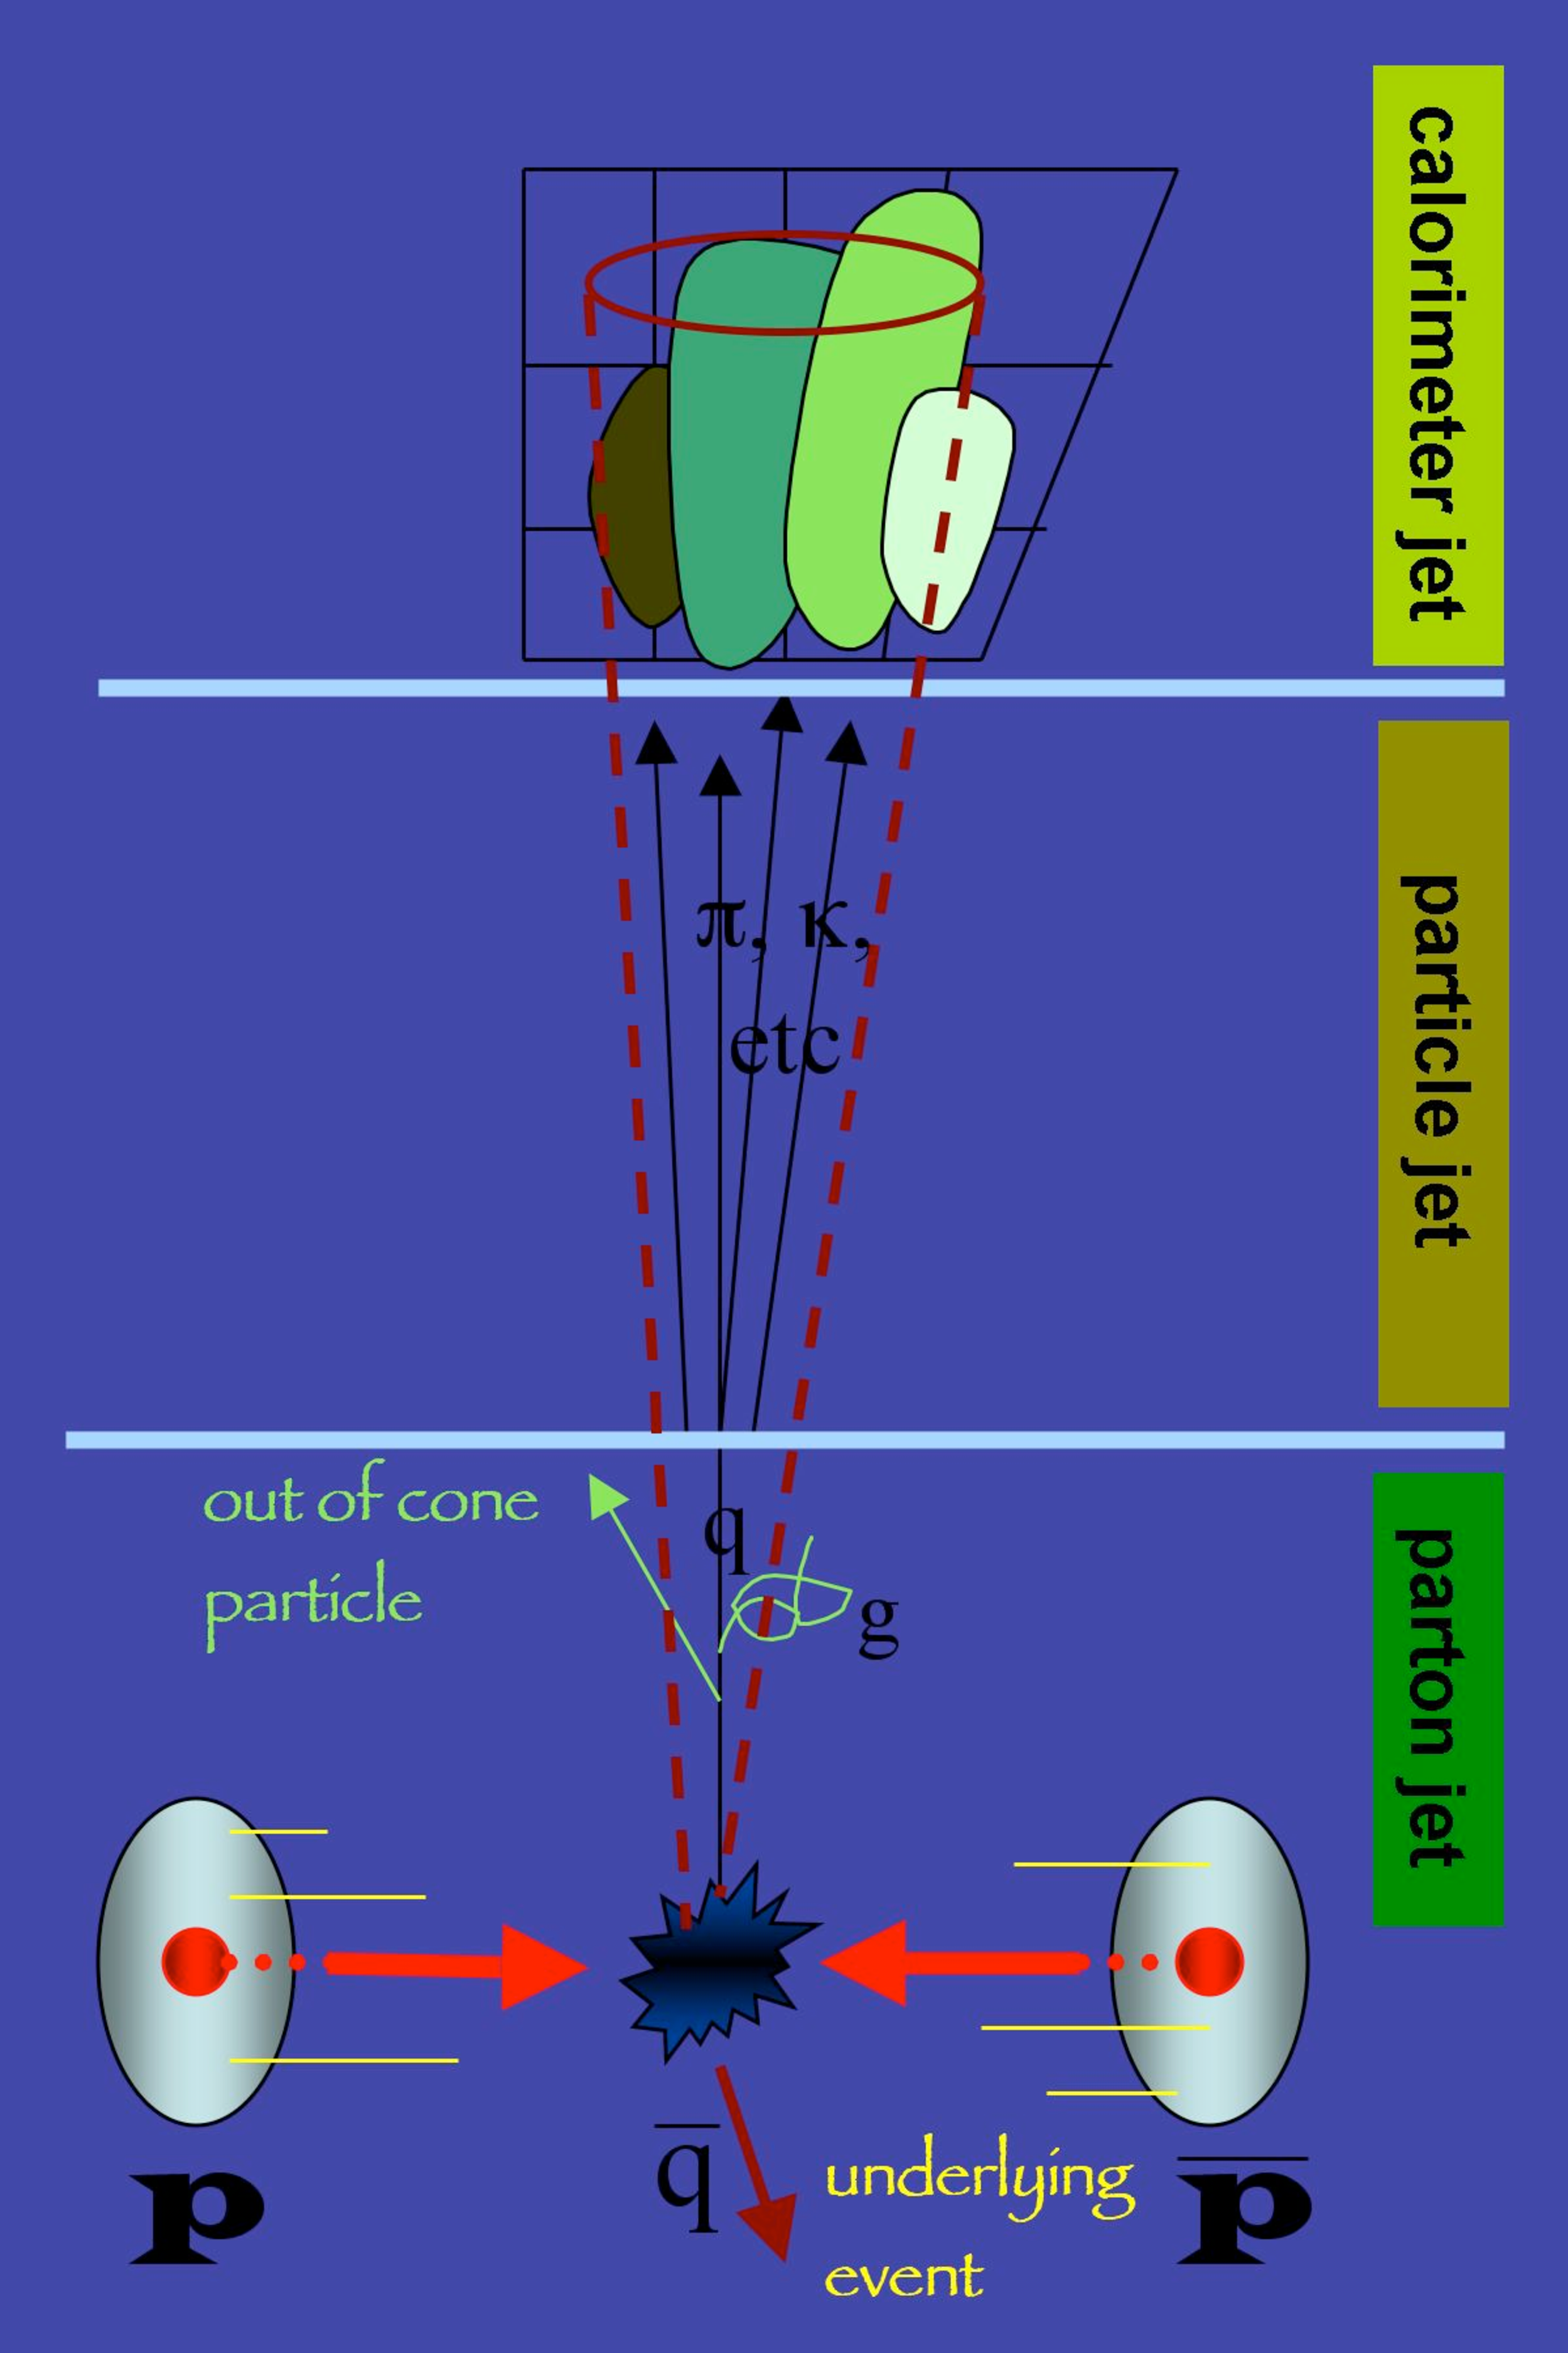
\includegraphics[scale=0.14]{PartonJetPartcleJetAndCalJet.pdf}
\caption{Evolution of a jet. A parton jet is formed soon after the hard collision. A particle jet (or hadron-level jet) is formed after quarks and gluons hadronize into colorless particles. Finally, a calorimeter jet or (detector-level jet) is actually measured and observed in the detector using a clustering algorithm.}
\label{fig:jetdefinition}
\end{centering}
\end{figure}

\begin{figure}[p]
 \centering
 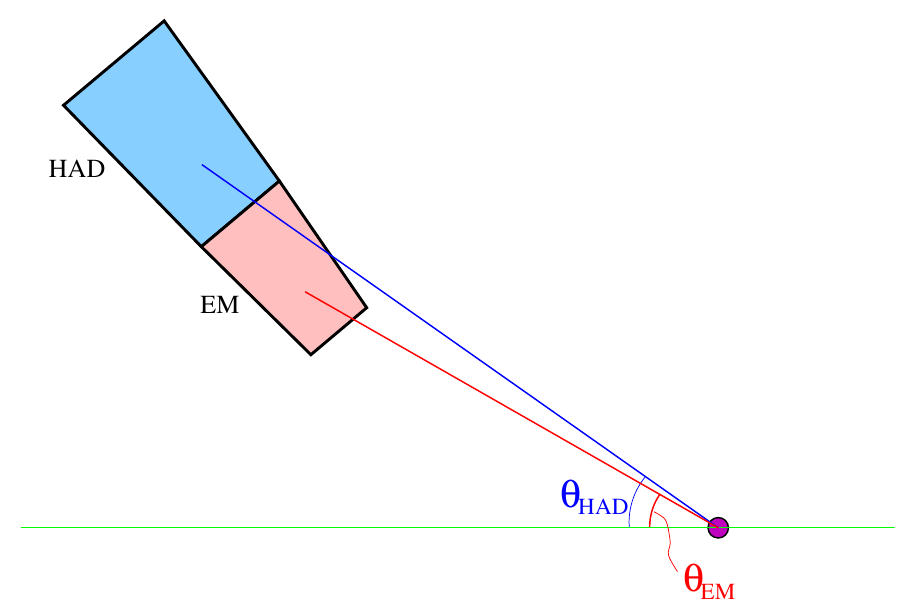
\includegraphics[scale=.5]{./JetClust_SingleCaloTower.png}
 % JetClust_SingleCaloTower.png: 903x613 pixel, 96dpi, 23.89x16.22 cm, bb=0 0 677 460
 \caption{Schematic of a single CDF calorimeter tower used in jet clustering.}
 \label{fig:jetClus_CaloTower}
\end{figure}


Identification of jets follows the same general concepts as described at the beginning of photon identification in Section~\ref{sec:photon_identification}. The energy of a jet is calculated from the energy deposited in the calorimeter towers (both EM and HAD) with the aid of clustering algorithms. There are many different clustering algorithms and each has its limitations. For this study, jets are clustered using a cone algorithm with a fixed cone size in which the center of the jet is defined as ($\eta^{jet}$, $\phi^{jet}$) and the size of the jet cone is $R = \sqrt{(\eta^{tower} - \eta^{jet})^{2} + (\phi^{tower} - \phi^{jet})^{2}} = 0.4$ (other options are 0.7 and 1.0). The jet clustering algorithm starts by identifying calorimeter towers with $E_{Ti}>1$~GeV to form seeds for jets, where $E_{Ti} = E_{i}\cdot\sin\theta _{i}$ is the transverse energy of a tower with respect to the $z$-position of the \ppbar interaction (see Fig.~\ref{fig:jetClus_CaloTower}), and the energy $E_{i}$ is the sum of the energies measured in the electromagnetic and hadronic compartments of that tower. The seed towers are sorted in order of decreasing $E_{Ti}$. Then, for each seed tower, towers within a radius $R$ of the seed tower's position are used to build clusters. The initial cluster transverse energy and the location of the cluster are calculated using the following definitions where $N_{tow}$ is the number of towers with $E_{T}>100$~MeV inside the radius $R$.
\begin{eqnarray}
 E^{jet}_{T} &=& \sum_{i=0}^{N_{tow}} E_{Ti}\\
 \phi^{jet} &=& \sum_{i=0}^{N_{tow}} \frac{E_{Ti}\phi_i}{E^{jet}_{T}}\\
 \eta^{jet} &=& \sum_{i=0}^{N_{tow}} \frac{E_{Ti}\eta_i}{E^{jet}_{T}}
\end{eqnarray}

For each cluster, this weighted average of the transverse energy in the cluster is used to identify the centroid of the cluster. Neighboring towers inside the cone with energies above the threshold are added and subtracted until a stable centroid is reached. Overlapping jets are merged if they overlap by more than the cutoff ($\sim$75\%). If the overlap is smaller, each tower in the overlap region is assigned to the nearest jets. The final jet energy, also known as \newterm{raw jet energy}, and momentum coordinates are computed from the final list of towers as described below.

\begin{eqnarray}
 E^{jet} &=& \sum_{i=0}^{N_{tow}} E_{i}\\
 p_{x}^{jet} &=& \sum_{i=0}^{N_{tow}} E_{i} \cdot \mathrm{sin}(\theta_{i}) \cdot \mathrm{cos}(\phi_{i})\\
 p_{y}^{jet} &=& \sum_{i=0}^{N_{tow}} E_{i} \cdot \mathrm{sin}(\theta_{i}) \cdot \mathrm{sin}(\phi_{i})
\end{eqnarray}

\begin{eqnarray}
p_{z}^{jet} &=& \sum_{i=0}^{N_{tow}} E_{i} \cdot \mathrm{cos}(\theta_{i})\\
p^{jet}_{T} &=& \sqrt{(p_{x}^{jet})^{2}+(p_{y}^{jet})^{2}}\\
\phi^{jet} &=& \mathrm{tan} (\frac{p_{y}^{jet}}{p_{x}^{jet}})\\
\mathrm{sin}(\theta^{jet}) &=& \frac{p^{jet}_{T}}{\sqrt{(p_{x}^{jet})^{2}+(p_{y}^{jet})^{2}+(p_{z}^{jet})^{2}}}\\
E_{T}^{jet} &=& E^{jet}\cdot\mathrm{sin}(\theta^{jet})
\end{eqnarray}


\section{Jet Energy Corrections}
The energies of clustered jets are corrected for detector effects, calorimeter response, and for physics-related effects. The sequence of corrections is described in the following section and described in detail elsewhere \cite{pap:JetCorrections}. % I have taken the text in the middle verbatim from the the citation, from section jet clustering.

\vspace{-0.01\textheight}
\begin{singlespace}
\begin{enumerate}
\item{\BUbf{$\eta$-dependent Corrections} --- Also known as the \newterm{relative corrections}, the $\eta$-dependent corrections are applied to raw jet energies to make the calorimeter response to jet energies uniform in $\eta$. These corrections are derived by measuring the transverse energy balance in dijet events. One jet is required to be in the central region of the detector (\etaregion{0.2}{0.6}) and the other is used as a probe. This is because the central calorimeter has a better resolution and is better understood. Figure~\ref{fig:JetCorrections_EtaDependence} shows the scale of this correction for different detector regions. Different corrections for data and simulated data samples are derived.}

\item{\BUbf{Corrections for Multiple \ppbar Interactions} --- At higher luminosity, more than one \ppbar interaction in a beam crossing can occur (see Chapter~\ref{chp:MCSimulation}). This may add extra energy to the clustering cone that needs to be removed. In such events, there will be more than one primary vertex. The corrections are derived using minimum bias data\footnote{These events are collected using a minimum bias trigger which requires hits in the east and west CLC detectors and no other requirements.} by measuring the transverse energy deposited in a random cone and parameterizing it as a function of the number of vertices in the event (see Fig.~\ref{fig:JetCorrections_MI}).}

\item{\BUbf{Absolute Corrections} --- After jet energies are corrected for $\eta$-dependence, they are further corrected for any non-linearity and energy loss in the uninstrumented regions of the central calorimeter. The absolute jet energy scale of the central calorimeter is determined by \pythiaText dijet \MC events. The observed calorimeter cluster energy (jet) is compared to the stable hadron-level jet which is identified using the same clustering algorithm. The scale of this correction is shown in Fig.~\ref{fig:JetCorrections_Absolute}.}

\item{\BUbf{Underlying Event Corrections} --- The underlying event (UE) is defined as the energy associated with the spectator partons in a hard collision event (see Chapter~\ref{chp:MCSimulation}). This extra energy needs to be subtracted from the jet energy in order to compare with the theoretical predictions involving only the hard collision. This correction is derived in a similar way to the corrections for multiple \ppbar interactions, using minimum bias data, but using events with only one primary vertex. The scale of these corrections for different clustering cone sizes is shown in Table~\ref{tab:JetCorrections_UE}.}

% \item{{\bf Out-of-cone Corrections} --- It is possible for a parton to radiate particles whose energy falls outside of the clustering cone. This out-of-cone energy needs to be added back to the particle jet. This corrects the particle jet energy for leakage of radiation outside the clustering cone used for jet definition and takes it back to \newterm{parent parton energy} (parton-level jet), which can be compared to theoretical predictions. The correction is derived using dijet \pythiaText \MC events. Hadron-level jets are matched to partons by requiring $\Delta R<0.1$ and is parameterized as a function of the hadron level jet energy (see Fig.~\ref{fig:JetCorrections_OOC}).}
\end{enumerate}
\end{singlespace}

\begin{figure}[p]
 \centering
 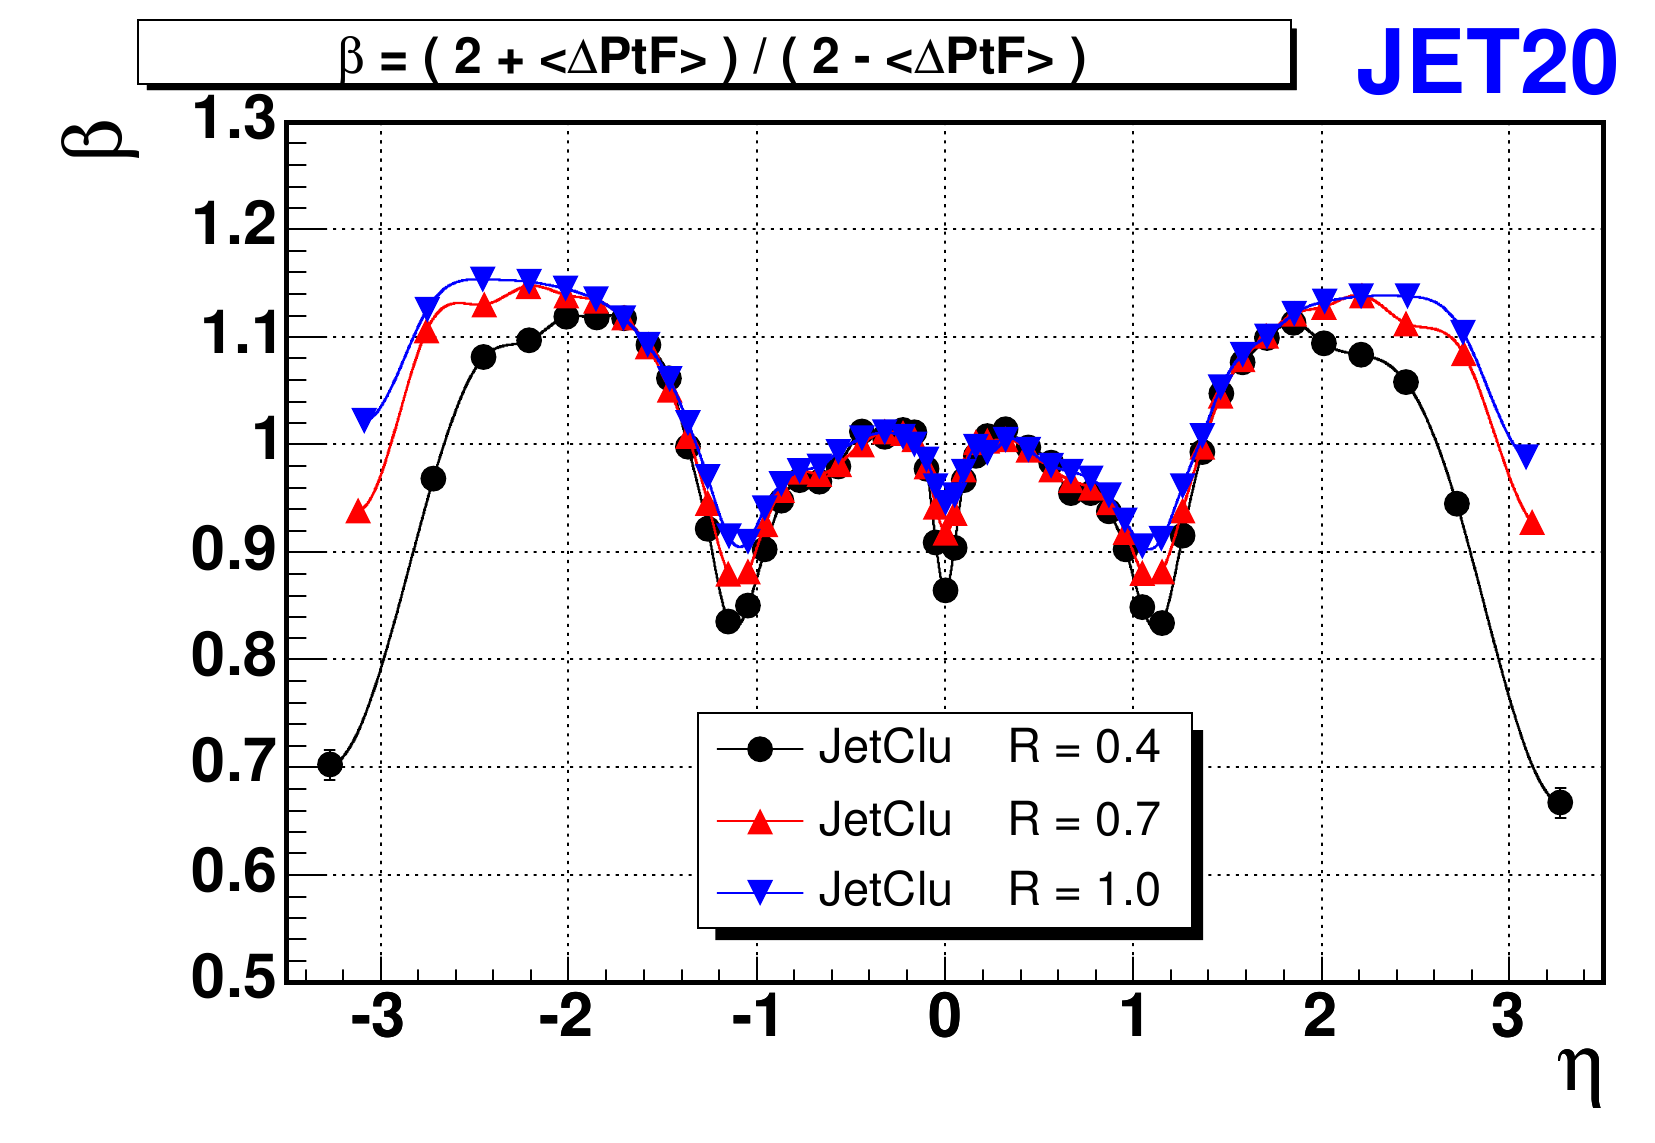
\includegraphics[scale=0.35,keepaspectratio=true]{./JetCorrections_EtaDependence.png}
 % JetCorrections_EtaDependence.png: 1655x1143 pixel, 96dpi, 43.78x30.24 cm, bb=0 0 1241 857
\caption{$\eta$-dependent corrections for jet energies: \pt balancing in dijet events as a function of $\eta$ for three different clustering cone sizes.}
 \label{fig:JetCorrections_EtaDependence}
\end{figure}

\begin{figure}[p]
 \centering
\subfigure{
 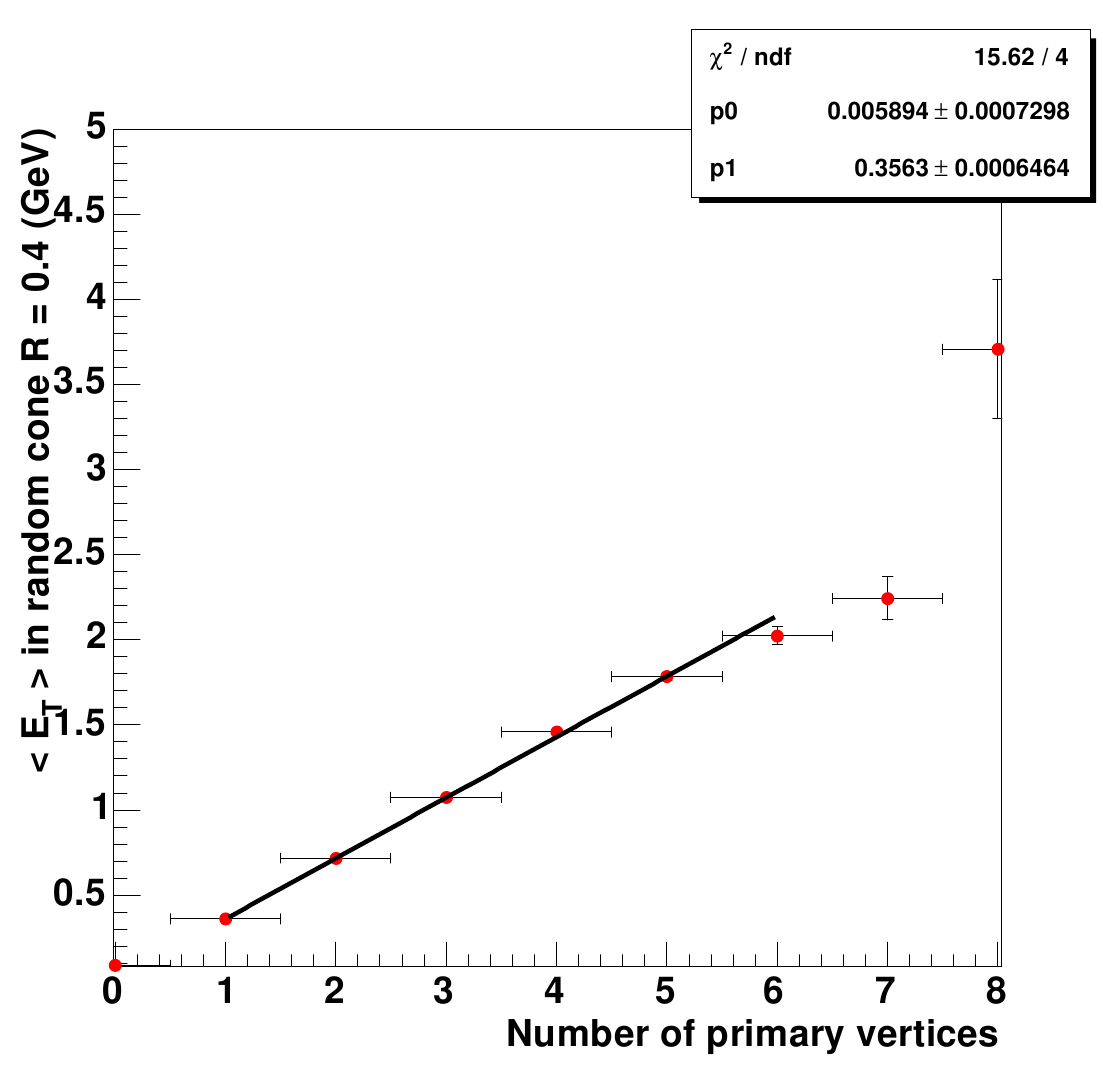
\includegraphics[scale=0.25,keepaspectratio=true]{./JetCorrections_MI_cone4.png}
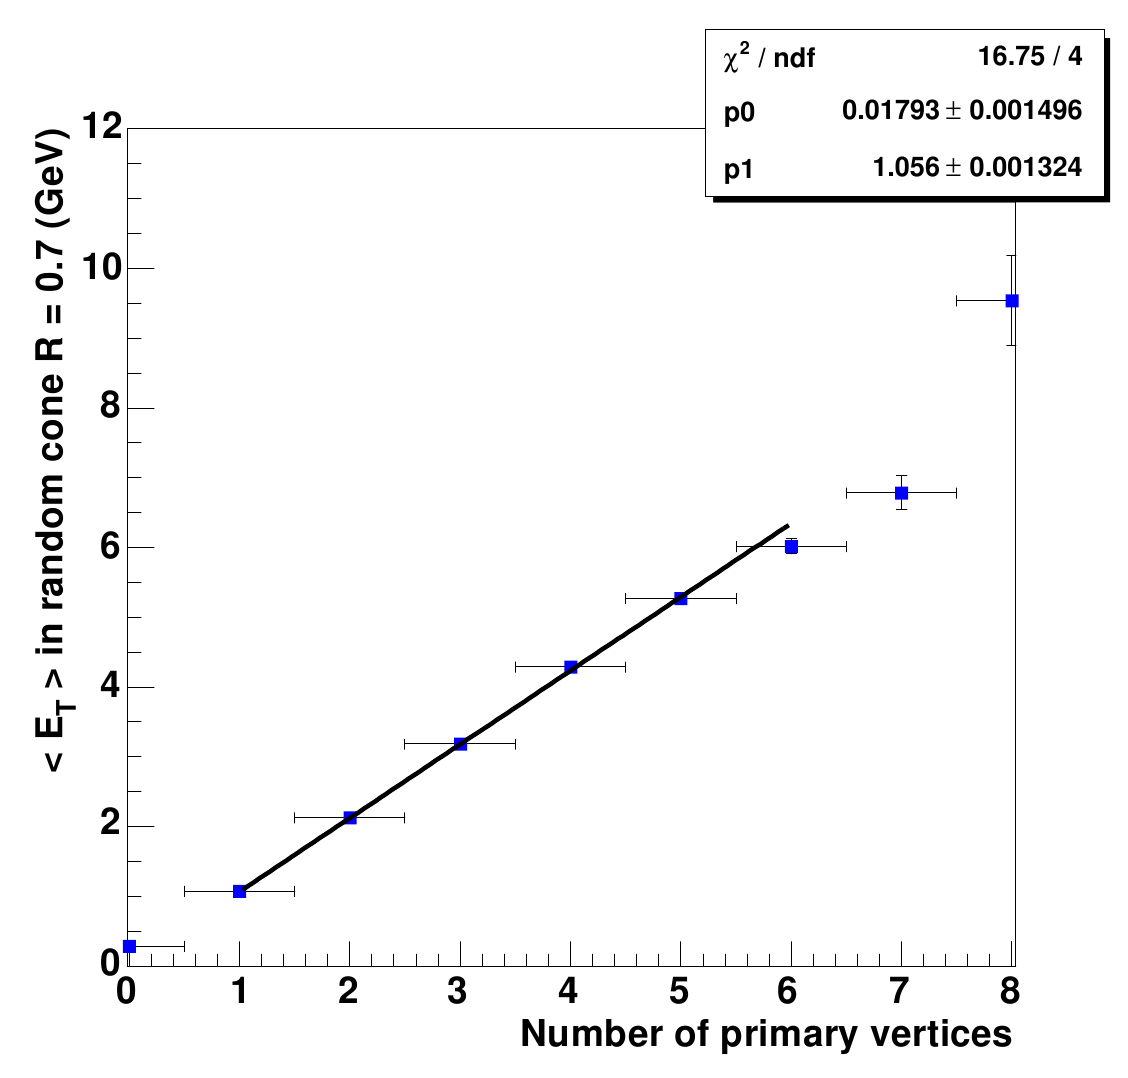
\includegraphics[scale=0.25,keepaspectratio=true]{./JetCorrections_MI_cone7.png}
}
\caption{Jet energy correction for multiple \ppbar interactions as a function of the number of vertices in the event for a clustering cone size of $R=0.4$ (left) and $R=0.7$ (right).}
 \label{fig:JetCorrections_MI}
\end{figure}

\begin{figure}[p]
 \centering
 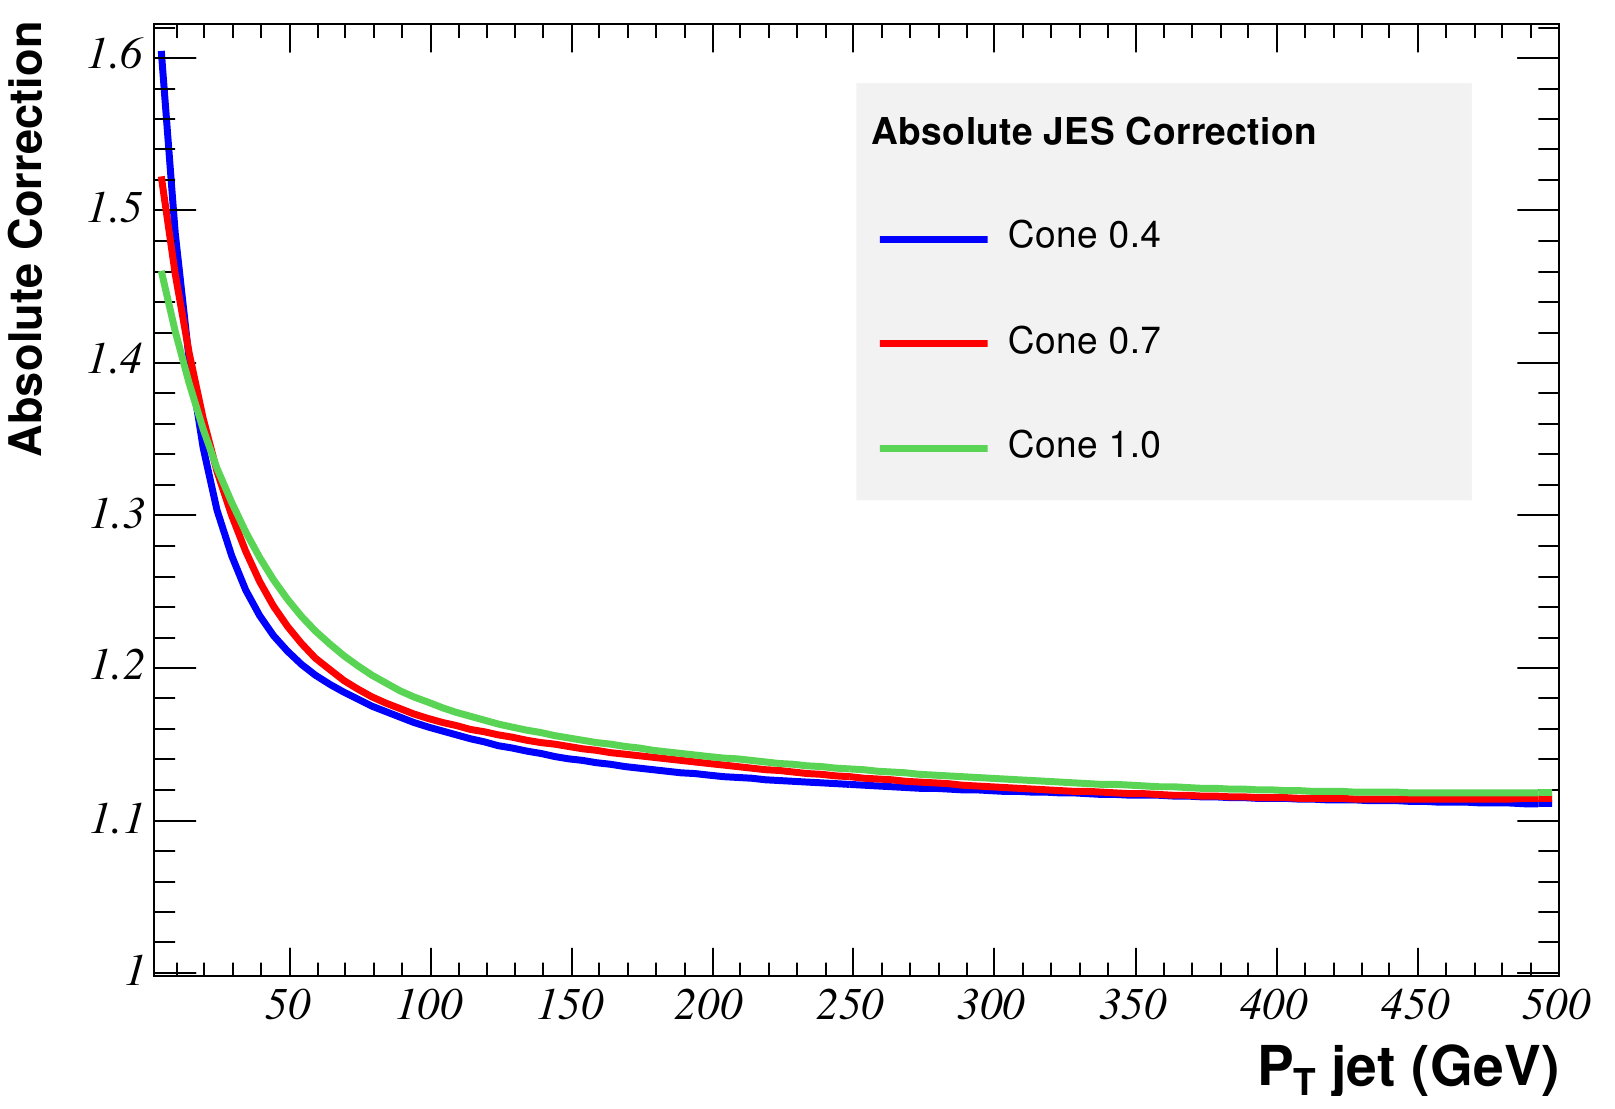
\includegraphics[scale=0.35,keepaspectratio=true]{./JetCorrections_Absolute.png}
 % JetCorrections_Absolute.png: 1615x1109 pixel, 96dpi, 42.72x29.34 cm, bb=0 0 1211 832
 \caption{Absolute jet energy scale corrections as a function of jet \pt for different clustering cone sizes.}
 \label{fig:JetCorrections_Absolute}
\end{figure}

\begin{table}[p]
\caption{Underlying event corrections to the jet energy for different clustering cone sizes.}
\label{tab:JetCorrections_UE}
\centering
 \begin{tabular}{cc}
\hline
\BUbf{Cone size} & \BUbf{Correction} \\
\hline
0.4 & 0.6~GeV\\
0.7 & 1.6~GeV\\
1.0 & 3.2~GeV\\
\hline
 \end{tabular}
\end{table}

% \begin{figure}[p]
%  \centering
%  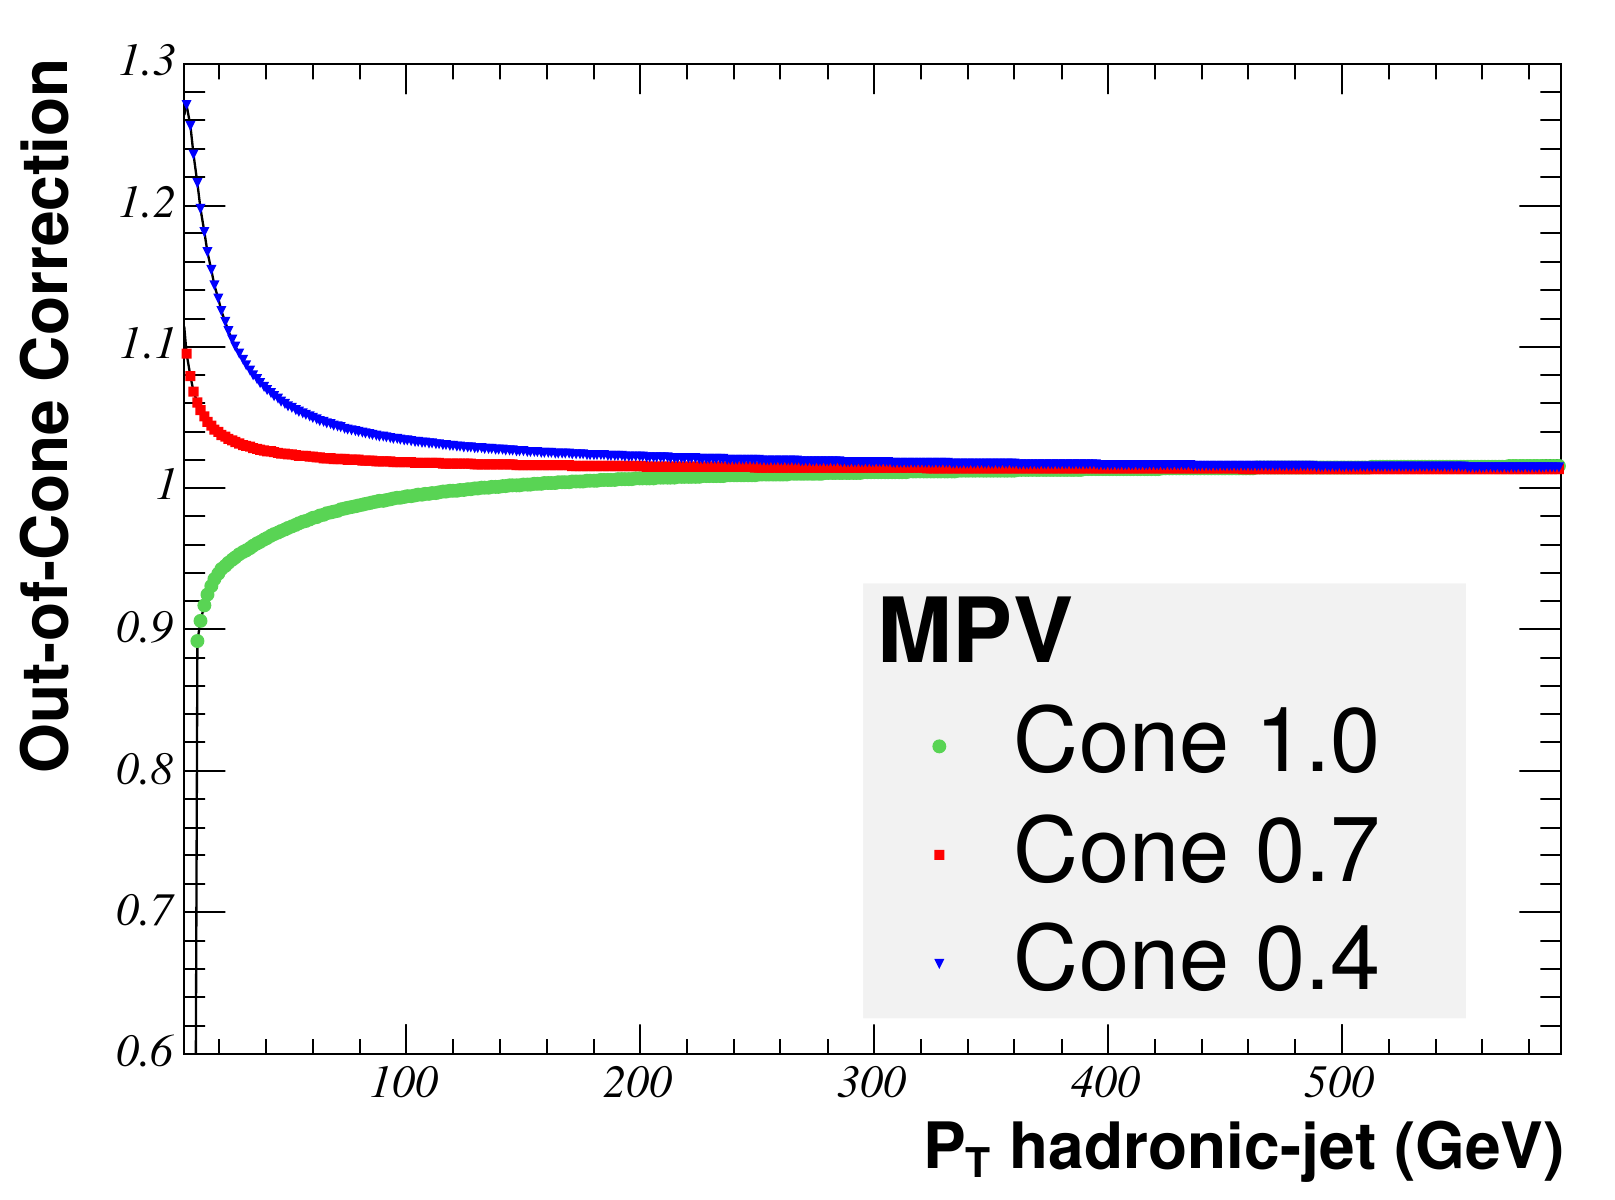
\includegraphics[scale=0.35]{./JetCorrections_OOC.png}
%  % JetCorrections_OOC.png: 1615x1200 pixel, 96dpi, 42.72x31.75 cm, bb=0 0 1211 900
%  \caption{Out-of-cone jet energy corrections as a function of hadron-level jet \pt for different clustering cone sizes.}
%  \label{fig:JetCorrections_OOC}
% \end{figure}

The corrections described above are applied to the measured (or raw) jet according to the following equation:
\begin{eqnarray}\nonumber
 P_{T}(R,P_{T},\eta) &=& (P_{T}^{raw}(R)\times f_{\eta}(R,P_{T},\eta)-MI(R))\times f_{jes}(R,P_{T})\\
& & -UE(R)+OOC(R,P_{T})
\end{eqnarray}
\noindent where $R$ is the clustering cone radius, $P_{T}$ is the measured energy in the cone, $\eta$ is the detector pseudorapidity of the jet, $f_{\eta}$ is the $\eta$-dependent correction, $MI$ is the correction for multiple \ppbar interactions, $f_{jes}$ is the central calorimeter jet energy scale, $UE$ is the correction for the underlying event, and $OOC$ is the out-of-cone correction. This can be further simplified and understood as
\begin{equation}
 P_{T}^{parton} = P_{T}^{particle}-UE+OOC
\end{equation}
\noindent where $P_{T}^{parton}$ is the transverse momentum of the original parton and $P_{T}^{particle}$ is the transverse momentum of the detector jet ($P_{T}^{raw}$) corrected for all detector effects and multiple \ppbar interactions.

It should be noted that all these corrections are derived on average. The systematic uncertainties of these corrections can range from few percent to $>$50\% depending on the energy of the jet. Also, the $OOC$ corrections are not necessary unless results need to be compared with the theory.

\section{Missing Transverse Energy (\met), $H_{T}$, and Invariant Mass}\label{sec:MetReconstruction}
The momenta of the colliding partons lie primarily along the $z$-axis and there is no significant energy in the transverse plane. Hence, the vector sum of transverse energies of particles produced in the collision should be zero. Any undetectable particles (like $\nu$) or energy mismeaurements will result in an energy imbalance in the transverse plane which is known as missing transverse energy (\met). \met is the hardest kinematic quantity to understand and model as it is a convolution of many effects, like the calorimeter response to different particles, primary vertex selection, etc. (See Appendix~\ref{app:MetModel} for more details of other effects on the \met measurement.)

The initial calculation of \met (\metRaw) assumes $x=y=z=0$ as the primary collision point. For analysis purposes it is a standard practice to use the \met calculated at the highest-sum-\pt ($\textstyle \sum\pt$) vertex. The highest-$\textstyle \sum \pt$ vertex is the vertex with the largest total \pt of all the tracks originating from the vertex. As corrections are applied to the photons, electrons, and jets in an event, the \met is also corrected accordingly (also known as \metCorr). The \met has two major components: real \met from undetected particles like $\nu$ and fake \met due to mismeasured energies of the particles. Because the energy resolution of the hadron calorimeter is poor compared to that of the EM calorimeter, fake \met arises mainly from mismeasured jets.

The variable $H_{T}$ measures the total energy in the transverse plane. It is the scalar sum of transverse energies of all the identified EM objects ($\gamma, e^{\pm}$), jets, and \met.

The invariant mass of two particles (in natural units) is defined as:
\begin{equation}
 M = \sqrt{(E_{1}+E_{2})^{2}-|\vec{p_{1}}+\vec{p_{2}}|^{2}}
\end{equation}
where $E_{i}$ and $\vec{p_{i}}$ correspond to the energy and the momentum of each particle, respectively.  In the case of two-particle decay, the invariant mass of the decay products gives the mass of the particle that decayed.  If, for example, a particle decays to a quark and antiquark which subsequently form two jets, the invariant mass of the two jets would give a measurement of the mass of the original particle.
